\section{(2, 2) Tree Graph State}
\label{sec:2_2_tree}

\begin{figure}
    \centering
    

\tikzset{every picture/.style={line width=0.75pt}} %set default line width to 0.75pt        

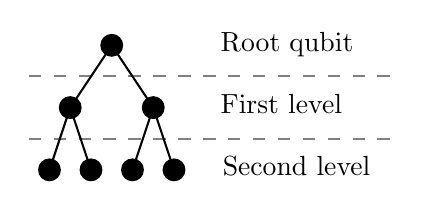
\begin{tikzpicture}[x=0.75pt,y=0.75pt,yscale=-1,xscale=1]
%uncomment if require: \path (0,300); %set diagram left start at 0, and has height of 300

%Straight Lines [id:da8426905590991587] 
\draw [color={rgb, 255:red, 128; green, 128; blue, 128 }  ,draw opacity=1 ] [dash pattern={on 4.5pt off 4.5pt}]  (60,85) -- (240,85) ;
%Straight Lines [id:da5406148798931413] 
\draw [color={rgb, 255:red, 128; green, 128; blue, 128 }  ,draw opacity=1 ] [dash pattern={on 4.5pt off 4.5pt}]  (60,55) -- (240,55) ;
%Straight Lines [id:da0310472865739988] 
\draw    (80,70) -- (90,100) ;
%Straight Lines [id:da44724908569705224] 
\draw    (80,70) -- (100,40) ;
%Shape: Circle [id:dp9646050192410193] 
\draw  [fill={rgb, 255:red, 0; green, 0; blue, 0 }  ,fill opacity=1 ] (95,40) .. controls (95,37.24) and (97.24,35) .. (100,35) .. controls (102.76,35) and (105,37.24) .. (105,40) .. controls (105,42.76) and (102.76,45) .. (100,45) .. controls (97.24,45) and (95,42.76) .. (95,40) -- cycle ;
%Shape: Circle [id:dp9987430184128605] 
\draw  [fill={rgb, 255:red, 0; green, 0; blue, 0 }  ,fill opacity=1 ] (105,100) .. controls (105,97.24) and (107.24,95) .. (110,95) .. controls (112.76,95) and (115,97.24) .. (115,100) .. controls (115,102.76) and (112.76,105) .. (110,105) .. controls (107.24,105) and (105,102.76) .. (105,100) -- cycle ;
%Shape: Circle [id:dp5327923177036115] 
\draw  [fill={rgb, 255:red, 0; green, 0; blue, 0 }  ,fill opacity=1 ] (125,100) .. controls (125,97.24) and (127.24,95) .. (130,95) .. controls (132.76,95) and (135,97.24) .. (135,100) .. controls (135,102.76) and (132.76,105) .. (130,105) .. controls (127.24,105) and (125,102.76) .. (125,100) -- cycle ;
%Shape: Circle [id:dp07874792740386194] 
\draw  [fill={rgb, 255:red, 0; green, 0; blue, 0 }  ,fill opacity=1 ] (115,70) .. controls (115,67.24) and (117.24,65) .. (120,65) .. controls (122.76,65) and (125,67.24) .. (125,70) .. controls (125,72.76) and (122.76,75) .. (120,75) .. controls (117.24,75) and (115,72.76) .. (115,70) -- cycle ;
%Shape: Circle [id:dp827553292195197] 
\draw  [fill={rgb, 255:red, 0; green, 0; blue, 0 }  ,fill opacity=1 ] (65,100) .. controls (65,97.24) and (67.24,95) .. (70,95) .. controls (72.76,95) and (75,97.24) .. (75,100) .. controls (75,102.76) and (72.76,105) .. (70,105) .. controls (67.24,105) and (65,102.76) .. (65,100) -- cycle ;
%Shape: Circle [id:dp9737971224660668] 
\draw  [fill={rgb, 255:red, 0; green, 0; blue, 0 }  ,fill opacity=1 ] (85,100) .. controls (85,97.24) and (87.24,95) .. (90,95) .. controls (92.76,95) and (95,97.24) .. (95,100) .. controls (95,102.76) and (92.76,105) .. (90,105) .. controls (87.24,105) and (85,102.76) .. (85,100) -- cycle ;
%Shape: Circle [id:dp3888180938045467] 
\draw  [fill={rgb, 255:red, 0; green, 0; blue, 0 }  ,fill opacity=1 ] (75,70) .. controls (75,67.24) and (77.24,65) .. (80,65) .. controls (82.76,65) and (85,67.24) .. (85,70) .. controls (85,72.76) and (82.76,75) .. (80,75) .. controls (77.24,75) and (75,72.76) .. (75,70) -- cycle ;
%Straight Lines [id:da09087177582110562] 
\draw    (80,70) -- (70,100) ;
%Straight Lines [id:da9701309593546271] 
\draw    (100,40) -- (120,70) ;
%Straight Lines [id:da7485547301936679] 
\draw    (110,100) -- (120,70) ;
%Straight Lines [id:da005037302745795835] 
\draw    (120,70) -- (130,100) ;

% Text Node
\draw (151,32) node [anchor=north west][inner sep=0.75pt]   [align=left] {Root qubit};
% Text Node
\draw (151,62) node [anchor=north west][inner sep=0.75pt]   [align=left] {First level};
% Text Node
\draw (152,92) node [anchor=north west][inner sep=0.75pt]   [align=left] {Second level};


\end{tikzpicture}
    \vspace{-1cm}
    \caption{Representation of $(2, 2)$ tree graph state}
    \label{fig:2_2_graph}
\end{figure}

The term \emph{$(n, m)$ tree graph state} refers to a tree structure where the initial qubit, known as the root qubit, links to $n$ other qubits, each of which is connected to $m$ additional qubits.
Specifically, we'll focus on examining a $(2, 2)$ tree graph state, visually represented in \cref{fig:2_2_graph}.

The tree graph state holds importance in quantum repeater protocols as it allows encoding a qubit at the root node.
This enables qubit transmission even if some photons are lost.
This resilience, requiring only a subset of essential photons for loss correction \cite{Why_tree_graph_state}, ensures reliable communication despite potential losses.

Hence, it is crucial to create the tree graph state while ensuring the root remains associated with one of our qubits.
This is necessary as we need the root qubit accessible for Bell state measurements, enabling us to encode the intended state for transmission.

We will begin by outlining the protocol employed to create the initial branch of the $(2, 2)$ tree graph state.
Initially, we generate the root qubit for the tree state using a straightforward $\pi/2$ $y$ rotation.
In the circuit diagram, the first quantum wire signifies the root qubit, representing a physical qubit in our device. The subsequent quantum wire represents the second physical qubit, while the remaining wires symbolize flying photons.
\begin{equation}
\label{eq:1_branch_implementation}
    \begin{quantikz}
      \lstick{$S_1 \rightarrow \ket{0}_1$} & \gate{Y_+}\slice[style=black]{\textbf{(a)}}  & \qw      & \qw                  & \ctrl{1}   & \qw   & \qw      & \qw                 & \qw \\
      \lstick{$S_2 \rightarrow \ket{0}_2$} & \gate{Y_+} & \ctrl{2} & \gate{Y_-}\slice[style=black]{\textbf{(b)}}  & \control{}\slice[style=black]{\textbf{(c)}} & \qw   & \ctrl{1} & \gate{Y_+}\slice[style=black]{\textbf{(d)}} & \qw \\
      \lstick{$\ket{0}_3$} & \qw                 & \qw      & \qw                  & \qw        & \qw   & \targ{}  & \qw                 & \qw \\
      \lstick{$\ket{0}_4$} & \qw                 & \targ{}  & \qw                  & \qw        & \qw   & \qw      & \qw                 & \qw 
    \end{quantikz}
\end{equation}

\begin{figure}
    \centering
    

\tikzset{every picture/.style={line width=0.75pt}} %set default line width to 0.75pt        

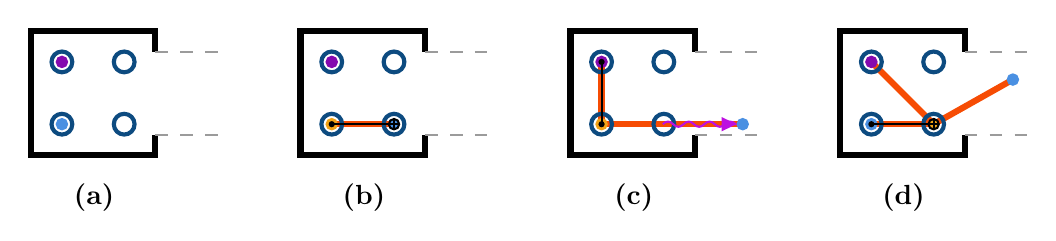
\begin{tikzpicture}[x=0.75pt,y=0.75pt,yscale=-1,xscale=1]
%uncomment if require: \path (0,134); %set diagram left start at 0, and has height of 134

%Shape: Circle [id:dp8634696649139634] 
\draw  [color={rgb, 255:red, 13; green, 75; blue, 128 }  ,draw opacity=1 ][line width=1.5]  (30,35) .. controls (30,32.24) and (32.24,30) .. (35,30) .. controls (37.76,30) and (40,32.24) .. (40,35) .. controls (40,37.76) and (37.76,40) .. (35,40) .. controls (32.24,40) and (30,37.76) .. (30,35) -- cycle ;
%Shape: Circle [id:dp3171229884283615] 
\draw  [color={rgb, 255:red, 13; green, 75; blue, 128 }  ,draw opacity=1 ][line width=1.5]  (30,65) .. controls (30,62.24) and (32.24,60) .. (35,60) .. controls (37.76,60) and (40,62.24) .. (40,65) .. controls (40,67.76) and (37.76,70) .. (35,70) .. controls (32.24,70) and (30,67.76) .. (30,65) -- cycle ;
%Shape: Circle [id:dp8674284799713297] 
\draw  [color={rgb, 255:red, 13; green, 75; blue, 128 }  ,draw opacity=1 ][line width=1.5]  (60,65) .. controls (60,62.24) and (62.24,60) .. (65,60) .. controls (67.76,60) and (70,62.24) .. (70,65) .. controls (70,67.76) and (67.76,70) .. (65,70) .. controls (62.24,70) and (60,67.76) .. (60,65) -- cycle ;
%Shape: Circle [id:dp13408530876145808] 
\draw  [color={rgb, 255:red, 13; green, 75; blue, 128 }  ,draw opacity=1 ][line width=1.5]  (60,35) .. controls (60,32.24) and (62.24,30) .. (65,30) .. controls (67.76,30) and (70,32.24) .. (70,35) .. controls (70,37.76) and (67.76,40) .. (65,40) .. controls (62.24,40) and (60,37.76) .. (60,35) -- cycle ;
%Shape: Square [id:dp47099491834906715] 
\draw  [line width=2.25]  (20,20) -- (80,20) -- (80,80) -- (20,80) -- cycle ;
%Straight Lines [id:da0834144987419978] 
\draw [color={rgb, 255:red, 255; green, 255; blue, 255 }  ,draw opacity=1 ][line width=3]    (80,30) -- (80,70) ;

%Shape: Circle [id:dp5113434790777113] 
\draw  [color={rgb, 255:red, 132; green, 9; blue, 175 }  ,draw opacity=1 ][fill={rgb, 255:red, 132; green, 9; blue, 175 }  ,fill opacity=1 ] (32.5,35) .. controls (32.5,33.62) and (33.62,32.5) .. (35,32.5) .. controls (36.38,32.5) and (37.5,33.62) .. (37.5,35) .. controls (37.5,36.38) and (36.38,37.5) .. (35,37.5) .. controls (33.62,37.5) and (32.5,36.38) .. (32.5,35) -- cycle ;
%Straight Lines [id:da46112915361915263] 
\draw [color={rgb, 255:red, 155; green, 155; blue, 155 }  ,draw opacity=1 ] [dash pattern={on 4.5pt off 4.5pt}]  (80,30) -- (110,30) ;
%Straight Lines [id:da9498457389457537] 
\draw [color={rgb, 255:red, 155; green, 155; blue, 155 }  ,draw opacity=1 ] [dash pattern={on 4.5pt off 4.5pt}]  (80,70) -- (110,70) ;
%Shape: Circle [id:dp9873280063938384] 
\draw  [color={rgb, 255:red, 74; green, 144; blue, 226 }  ,draw opacity=1 ][fill={rgb, 255:red, 74; green, 144; blue, 226 }  ,fill opacity=1 ] (32.5,65) .. controls (32.5,63.62) and (33.62,62.5) .. (35,62.5) .. controls (36.38,62.5) and (37.5,63.62) .. (37.5,65) .. controls (37.5,66.38) and (36.38,67.5) .. (35,67.5) .. controls (33.62,67.5) and (32.5,66.38) .. (32.5,65) -- cycle ;
%Shape: Circle [id:dp6431718269187471] 
\draw  [color={rgb, 255:red, 132; green, 9; blue, 175 }  ,draw opacity=1 ][fill={rgb, 255:red, 132; green, 9; blue, 175 }  ,fill opacity=1 ] (162.5,35) .. controls (162.5,33.62) and (163.62,32.5) .. (165,32.5) .. controls (166.38,32.5) and (167.5,33.62) .. (167.5,35) .. controls (167.5,36.38) and (166.38,37.5) .. (165,37.5) .. controls (163.62,37.5) and (162.5,36.38) .. (162.5,35) -- cycle ;
%Shape: Circle [id:dp21383549781911027] 
\draw  [color={rgb, 255:red, 13; green, 75; blue, 128 }  ,draw opacity=1 ][line width=1.5]  (160,35) .. controls (160,32.24) and (162.24,30) .. (165,30) .. controls (167.76,30) and (170,32.24) .. (170,35) .. controls (170,37.76) and (167.76,40) .. (165,40) .. controls (162.24,40) and (160,37.76) .. (160,35) -- cycle ;
%Shape: Circle [id:dp3789153251551227] 
\draw  [color={rgb, 255:red, 13; green, 75; blue, 128 }  ,draw opacity=1 ][line width=1.5]  (190,35) .. controls (190,32.24) and (192.24,30) .. (195,30) .. controls (197.76,30) and (200,32.24) .. (200,35) .. controls (200,37.76) and (197.76,40) .. (195,40) .. controls (192.24,40) and (190,37.76) .. (190,35) -- cycle ;
%Shape: Square [id:dp28884126483287875] 
\draw  [line width=2.25]  (150,20) -- (210,20) -- (210,80) -- (150,80) -- cycle ;
%Straight Lines [id:da7068966502224133] 
\draw [color={rgb, 255:red, 255; green, 255; blue, 255 }  ,draw opacity=1 ][line width=3]    (210,30) -- (210,70) ;

%Straight Lines [id:da5803960409811918] 
\draw [color={rgb, 255:red, 155; green, 155; blue, 155 }  ,draw opacity=1 ] [dash pattern={on 4.5pt off 4.5pt}]  (210,30) -- (240,30) ;
%Straight Lines [id:da7547530202356005] 
\draw [color={rgb, 255:red, 155; green, 155; blue, 155 }  ,draw opacity=1 ] [dash pattern={on 4.5pt off 4.5pt}]  (210,70) -- (240,70) ;
%Straight Lines [id:da6849475869613678] 
\draw [color={rgb, 255:red, 246; green, 76; blue, 4 }  ,draw opacity=1 ][line width=2.25]    (165,65) -- (195,65) ;
%Shape: Circle [id:dp7155137713689077] 
\draw  [color={rgb, 255:red, 241; green, 163; blue, 23 }  ,draw opacity=1 ][fill={rgb, 255:red, 241; green, 163; blue, 23 }  ,fill opacity=1 ] (162.5,65) .. controls (162.5,63.62) and (163.62,62.5) .. (165,62.5) .. controls (166.38,62.5) and (167.5,63.62) .. (167.5,65) .. controls (167.5,66.38) and (166.38,67.5) .. (165,67.5) .. controls (163.62,67.5) and (162.5,66.38) .. (162.5,65) -- cycle ;
%Shape: Circle [id:dp2190211775758546] 
\draw  [color={rgb, 255:red, 0; green, 0; blue, 0 }  ,draw opacity=1 ][fill={rgb, 255:red, 74; green, 144; blue, 226 }  ,fill opacity=1 ] (192.5,65) .. controls (192.5,63.62) and (193.62,62.5) .. (195,62.5) .. controls (196.38,62.5) and (197.5,63.62) .. (197.5,65) .. controls (197.5,66.38) and (196.38,67.5) .. (195,67.5) .. controls (193.62,67.5) and (192.5,66.38) .. (192.5,65) -- cycle ;
%Straight Lines [id:da5019530038163004] 
\draw    (195,62.5) -- (195,68) ;
%Straight Lines [id:da023533720970719596] 
\draw    (197.5,65) -- (192.5,65) ;
%Shape: Circle [id:dp463883226646705] 
\draw  [draw opacity=0][fill={rgb, 255:red, 0; green, 0; blue, 0 }  ,fill opacity=1 ] (163.5,65) .. controls (163.5,64.17) and (164.17,63.5) .. (165,63.5) .. controls (165.83,63.5) and (166.5,64.17) .. (166.5,65) .. controls (166.5,65.83) and (165.83,66.5) .. (165,66.5) .. controls (164.17,66.5) and (163.5,65.83) .. (163.5,65) -- cycle ;
%Shape: Circle [id:dp2941797335933385] 
\draw  [color={rgb, 255:red, 13; green, 75; blue, 128 }  ,draw opacity=1 ][line width=1.5]  (190,65) .. controls (190,62.24) and (192.24,60) .. (195,60) .. controls (197.76,60) and (200,62.24) .. (200,65) .. controls (200,67.76) and (197.76,70) .. (195,70) .. controls (192.24,70) and (190,67.76) .. (190,65) -- cycle ;
%Shape: Circle [id:dp19508965820109148] 
\draw  [color={rgb, 255:red, 13; green, 75; blue, 128 }  ,draw opacity=1 ][line width=1.5]  (160,65) .. controls (160,62.24) and (162.24,60) .. (165,60) .. controls (167.76,60) and (170,62.24) .. (170,65) .. controls (170,67.76) and (167.76,70) .. (165,70) .. controls (162.24,70) and (160,67.76) .. (160,65) -- cycle ;
%Straight Lines [id:da36230041238257815] 
\draw    (165,65) -- (195,65) ;
%Shape: Square [id:dp22566803032018268] 
\draw  [line width=2.25]  (280,20) -- (340,20) -- (340,80) -- (280,80) -- cycle ;
%Straight Lines [id:da8610306823319624] 
\draw [color={rgb, 255:red, 255; green, 255; blue, 255 }  ,draw opacity=1 ][line width=3]    (340,30) -- (340,70) ;

%Straight Lines [id:da9138577476417785] 
\draw [color={rgb, 255:red, 246; green, 76; blue, 4 }  ,draw opacity=1 ][line width=2.25]    (295,65) -- (363,65) ;
%Straight Lines [id:da9264747080487808] 
\draw [color={rgb, 255:red, 246; green, 76; blue, 4 }  ,draw opacity=1 ][line width=2.25]    (295,35) -- (295,65) ;
%Shape: Circle [id:dp826290588201388] 
\draw  [color={rgb, 255:red, 132; green, 9; blue, 175 }  ,draw opacity=1 ][fill={rgb, 255:red, 132; green, 9; blue, 175 }  ,fill opacity=1 ] (292.5,35) .. controls (292.5,33.62) and (293.62,32.5) .. (295,32.5) .. controls (296.38,32.5) and (297.5,33.62) .. (297.5,35) .. controls (297.5,36.38) and (296.38,37.5) .. (295,37.5) .. controls (293.62,37.5) and (292.5,36.38) .. (292.5,35) -- cycle ;
%Shape: Circle [id:dp9454665293887276] 
\draw  [color={rgb, 255:red, 13; green, 75; blue, 128 }  ,draw opacity=1 ][line width=1.5]  (290,35) .. controls (290,32.24) and (292.24,30) .. (295,30) .. controls (297.76,30) and (300,32.24) .. (300,35) .. controls (300,37.76) and (297.76,40) .. (295,40) .. controls (292.24,40) and (290,37.76) .. (290,35) -- cycle ;
%Shape: Circle [id:dp9678738407214998] 
\draw  [color={rgb, 255:red, 13; green, 75; blue, 128 }  ,draw opacity=1 ][line width=1.5]  (290,65) .. controls (290,62.24) and (292.24,60) .. (295,60) .. controls (297.76,60) and (300,62.24) .. (300,65) .. controls (300,67.76) and (297.76,70) .. (295,70) .. controls (292.24,70) and (290,67.76) .. (290,65) -- cycle ;
%Shape: Circle [id:dp11638652073637779] 
\draw  [color={rgb, 255:red, 13; green, 75; blue, 128 }  ,draw opacity=1 ][line width=1.5]  (320,65) .. controls (320,62.24) and (322.24,60) .. (325,60) .. controls (327.76,60) and (330,62.24) .. (330,65) .. controls (330,67.76) and (327.76,70) .. (325,70) .. controls (322.24,70) and (320,67.76) .. (320,65) -- cycle ;
%Shape: Circle [id:dp8846315373556948] 
\draw  [color={rgb, 255:red, 13; green, 75; blue, 128 }  ,draw opacity=1 ][line width=1.5]  (320,35) .. controls (320,32.24) and (322.24,30) .. (325,30) .. controls (327.76,30) and (330,32.24) .. (330,35) .. controls (330,37.76) and (327.76,40) .. (325,40) .. controls (322.24,40) and (320,37.76) .. (320,35) -- cycle ;
%Straight Lines [id:da15824455233757484] 
\draw [color={rgb, 255:red, 155; green, 155; blue, 155 }  ,draw opacity=1 ] [dash pattern={on 4.5pt off 4.5pt}]  (340,30) -- (370,30) ;
%Straight Lines [id:da08275578074384338] 
\draw [color={rgb, 255:red, 155; green, 155; blue, 155 }  ,draw opacity=1 ] [dash pattern={on 4.5pt off 4.5pt}]  (340,70) -- (370,70) ;
%Shape: Circle [id:dp4480793960053918] 
\draw  [color={rgb, 255:red, 241; green, 163; blue, 23 }  ,draw opacity=1 ][fill={rgb, 255:red, 241; green, 163; blue, 23 }  ,fill opacity=1 ] (292.5,65) .. controls (292.5,63.62) and (293.62,62.5) .. (295,62.5) .. controls (296.38,62.5) and (297.5,63.62) .. (297.5,65) .. controls (297.5,66.38) and (296.38,67.5) .. (295,67.5) .. controls (293.62,67.5) and (292.5,66.38) .. (292.5,65) -- cycle ;
%Shape: Circle [id:dp4701197125733043] 
\draw  [color={rgb, 255:red, 74; green, 144; blue, 226 }  ,draw opacity=1 ][fill={rgb, 255:red, 74; green, 144; blue, 226 }  ,fill opacity=1 ] (360.5,65) .. controls (360.5,63.62) and (361.62,62.5) .. (363,62.5) .. controls (364.38,62.5) and (365.5,63.62) .. (365.5,65) .. controls (365.5,66.38) and (364.38,67.5) .. (363,67.5) .. controls (361.62,67.5) and (360.5,66.38) .. (360.5,65) -- cycle ;
%Shape: Circle [id:dp36402367761201493] 
\draw  [draw opacity=0][fill={rgb, 255:red, 0; green, 0; blue, 0 }  ,fill opacity=1 ] (293.5,65) .. controls (293.5,64.17) and (294.17,63.5) .. (295,63.5) .. controls (295.83,63.5) and (296.5,64.17) .. (296.5,65) .. controls (296.5,65.83) and (295.83,66.5) .. (295,66.5) .. controls (294.17,66.5) and (293.5,65.83) .. (293.5,65) -- cycle ;
%Shape: Circle [id:dp7874046855771671] 
\draw  [draw opacity=0][fill={rgb, 255:red, 0; green, 0; blue, 0 }  ,fill opacity=1 ] (293.5,35) .. controls (293.5,34.17) and (294.17,33.5) .. (295,33.5) .. controls (295.83,33.5) and (296.5,34.17) .. (296.5,35) .. controls (296.5,35.83) and (295.83,36.5) .. (295,36.5) .. controls (294.17,36.5) and (293.5,35.83) .. (293.5,35) -- cycle ;
%Straight Lines [id:da2898778351352036] 
\draw    (295,35) -- (295,65) ;
%Straight Lines [id:da7752313531562761] 
\draw [color={rgb, 255:red, 189; green, 16; blue, 224 }  ,draw opacity=1 ]   (324.5,65) .. controls (326.17,63.33) and (327.83,63.33) .. (329.5,65) .. controls (331.17,66.67) and (332.83,66.67) .. (334.5,65) .. controls (336.17,63.33) and (337.83,63.33) .. (339.5,65) .. controls (341.17,66.67) and (342.83,66.67) .. (344.5,65) .. controls (346.17,63.33) and (347.83,63.33) .. (349.5,65) .. controls (351.17,66.67) and (352.83,66.67) .. (354.5,65) .. controls (356.17,63.33) and (357.83,63.33) .. (359.5,65) -- (360,65) -- (360,65) ;
%Straight Lines [id:da9446040288212432] 
\draw [color={rgb, 255:red, 189; green, 16; blue, 224 }  ,draw opacity=1 ]   (354.25,65) -- (357,65) ;
\draw [shift={(360,65)}, rotate = 180] [fill={rgb, 255:red, 189; green, 16; blue, 224 }  ,fill opacity=1 ][line width=0.08]  [draw opacity=0] (7.14,-3.43) -- (0,0) -- (7.14,3.43) -- cycle    ;
%Straight Lines [id:da4458315367718473] 
\draw [color={rgb, 255:red, 246; green, 76; blue, 4 }  ,draw opacity=1 ][line width=2.25]    (425,65) -- (455,65) ;
%Straight Lines [id:da6417507071495968] 
\draw [color={rgb, 255:red, 246; green, 76; blue, 4 }  ,draw opacity=1 ][line width=2.25]    (425,35) -- (455,65) ;
%Shape: Square [id:dp19892382898236483] 
\draw  [line width=2.25]  (410,20) -- (470,20) -- (470,80) -- (410,80) -- cycle ;
%Straight Lines [id:da8211154882339877] 
\draw [color={rgb, 255:red, 255; green, 255; blue, 255 }  ,draw opacity=1 ][line width=3]    (470,30) -- (470,70) ;

%Straight Lines [id:da1226594004392908] 
\draw [color={rgb, 255:red, 246; green, 76; blue, 4 }  ,draw opacity=1 ][line width=2.25]    (493.17,43.5) -- (455,65) ;
%Shape: Circle [id:dp25607475791662804] 
\draw  [color={rgb, 255:red, 132; green, 9; blue, 175 }  ,draw opacity=1 ][fill={rgb, 255:red, 132; green, 9; blue, 175 }  ,fill opacity=1 ] (422.5,35) .. controls (422.5,33.62) and (423.62,32.5) .. (425,32.5) .. controls (426.38,32.5) and (427.5,33.62) .. (427.5,35) .. controls (427.5,36.38) and (426.38,37.5) .. (425,37.5) .. controls (423.62,37.5) and (422.5,36.38) .. (422.5,35) -- cycle ;
%Shape: Circle [id:dp7472085667416201] 
\draw  [color={rgb, 255:red, 13; green, 75; blue, 128 }  ,draw opacity=1 ][line width=1.5]  (420,35) .. controls (420,32.24) and (422.24,30) .. (425,30) .. controls (427.76,30) and (430,32.24) .. (430,35) .. controls (430,37.76) and (427.76,40) .. (425,40) .. controls (422.24,40) and (420,37.76) .. (420,35) -- cycle ;
%Shape: Circle [id:dp6105247050154898] 
\draw  [color={rgb, 255:red, 13; green, 75; blue, 128 }  ,draw opacity=1 ][line width=1.5]  (420,65) .. controls (420,62.24) and (422.24,60) .. (425,60) .. controls (427.76,60) and (430,62.24) .. (430,65) .. controls (430,67.76) and (427.76,70) .. (425,70) .. controls (422.24,70) and (420,67.76) .. (420,65) -- cycle ;
%Shape: Circle [id:dp10304227171071978] 
\draw  [color={rgb, 255:red, 13; green, 75; blue, 128 }  ,draw opacity=1 ][line width=1.5]  (450,65) .. controls (450,62.24) and (452.24,60) .. (455,60) .. controls (457.76,60) and (460,62.24) .. (460,65) .. controls (460,67.76) and (457.76,70) .. (455,70) .. controls (452.24,70) and (450,67.76) .. (450,65) -- cycle ;
%Shape: Circle [id:dp4134298947687973] 
\draw  [color={rgb, 255:red, 13; green, 75; blue, 128 }  ,draw opacity=1 ][line width=1.5]  (450,35) .. controls (450,32.24) and (452.24,30) .. (455,30) .. controls (457.76,30) and (460,32.24) .. (460,35) .. controls (460,37.76) and (457.76,40) .. (455,40) .. controls (452.24,40) and (450,37.76) .. (450,35) -- cycle ;
%Straight Lines [id:da05857273260240248] 
\draw [color={rgb, 255:red, 155; green, 155; blue, 155 }  ,draw opacity=1 ] [dash pattern={on 4.5pt off 4.5pt}]  (470,30) -- (500,30) ;
%Straight Lines [id:da8515467099208363] 
\draw [color={rgb, 255:red, 155; green, 155; blue, 155 }  ,draw opacity=1 ] [dash pattern={on 4.5pt off 4.5pt}]  (470,70) -- (500,70) ;
%Shape: Circle [id:dp3385953242829104] 
\draw  [color={rgb, 255:red, 74; green, 144; blue, 226 }  ,draw opacity=1 ][fill={rgb, 255:red, 74; green, 144; blue, 226 }  ,fill opacity=1 ] (422.5,65) .. controls (422.5,63.62) and (423.62,62.5) .. (425,62.5) .. controls (426.38,62.5) and (427.5,63.62) .. (427.5,65) .. controls (427.5,66.38) and (426.38,67.5) .. (425,67.5) .. controls (423.62,67.5) and (422.5,66.38) .. (422.5,65) -- cycle ;
%Shape: Circle [id:dp6520838784850642] 
\draw  [color={rgb, 255:red, 0; green, 0; blue, 0 }  ,draw opacity=1 ][fill={rgb, 255:red, 241; green, 163; blue, 23 }  ,fill opacity=1 ] (452.5,65) .. controls (452.5,63.62) and (453.62,62.5) .. (455,62.5) .. controls (456.38,62.5) and (457.5,63.62) .. (457.5,65) .. controls (457.5,66.38) and (456.38,67.5) .. (455,67.5) .. controls (453.62,67.5) and (452.5,66.38) .. (452.5,65) -- cycle ;
%Straight Lines [id:da9256744917784654] 
\draw    (455,62) -- (455,67.5) ;
%Straight Lines [id:da28871784610038775] 
\draw    (425,65) -- (455,65) ;
%Straight Lines [id:da9178977220598342] 
\draw    (457.5,65) -- (452.5,65) ;
%Shape: Circle [id:dp7957363186924172] 
\draw  [draw opacity=0][fill={rgb, 255:red, 0; green, 0; blue, 0 }  ,fill opacity=1 ] (423.5,65) .. controls (423.5,64.17) and (424.17,63.5) .. (425,63.5) .. controls (425.83,63.5) and (426.5,64.17) .. (426.5,65) .. controls (426.5,65.83) and (425.83,66.5) .. (425,66.5) .. controls (424.17,66.5) and (423.5,65.83) .. (423.5,65) -- cycle ;
%Shape: Circle [id:dp6977350768470425] 
\draw  [color={rgb, 255:red, 74; green, 144; blue, 226 }  ,draw opacity=1 ][fill={rgb, 255:red, 74; green, 144; blue, 226 }  ,fill opacity=1 ] (490.67,43.5) .. controls (490.67,42.12) and (491.79,41) .. (493.17,41) .. controls (494.55,41) and (495.67,42.12) .. (495.67,43.5) .. controls (495.67,44.88) and (494.55,46) .. (493.17,46) .. controls (491.79,46) and (490.67,44.88) .. (490.67,43.5) -- cycle ;

% Text Node
\draw (50.5,92) node [anchor=north] [inner sep=0.75pt]   [align=left] {\textbf{(a)}};
% Text Node
\draw (180.5,92) node [anchor=north] [inner sep=0.75pt]   [align=left] {\textbf{(b)}};
% Text Node
\draw (310.5,92) node [anchor=north] [inner sep=0.75pt]   [align=left] {\textbf{(c)}};
% Text Node
\draw (440.5,92) node [anchor=north] [inner sep=0.75pt]   [align=left] {\textbf{(d)}};


\end{tikzpicture}
    \vspace{-1cm}
    \caption{Visual implementation of first branch of the $(2, 2)$ tree graph state}
    \label{fig:1_branch_tree}
\end{figure}

Fig.~\ref{fig:1_branch_tree} illustrates the visual progression occurring within the device.

Should we emit all nodes except for the root, we can replicate the process to generate the second and final branch of the intended quantum state.
The circuit illustrating the entire implementation of the tree graph state is presented below. 
Notably, the initial two quantum wires maintain their role as the first and second storage qubits.
Meanwhile, the remaining six wires signify the six additional vertices in the state, functioning as flying qubits in our configuration.
\begin{equation}
\label{eq:tree_implementation}
    \begin{quantikz}[column sep=0.4cm]
      \lstick{$\ket{0}_1$} & \gate{Y_+} & \qw & \qw & \ctrl{1} & \qw & \qw & \qw & \qw & \qw & \qw & \ctrl{1} & \qw & \qw & \qw \\
      \lstick{$\ket{0}_2$} & \gate{Y_+} & \ctrl{3} & \gate{Y_-} & \control{} & \ctrl{2} & \gate{Y_+} & \swap{1} & \gate{Y_+} & \ctrl{5} & \gate{Y_-} & \control{} & \ctrl{4} & \gate{Y_+} & \qw \\
      \lstick{$\ket{0}_3$} & \qw & \qw & \qw & \qw & \qw & \qw & \targX{} & \qw & \qw & \qw & \qw & \qw & \qw & \qw \\
      \lstick{$\ket{0}_4$} & \qw & \qw & \qw & \qw & \targ{} & \qw & \qw & \qw & \qw & \qw & \qw & \qw & \qw & \qw \\
      \lstick{$\ket{0}_5$} & \qw & \targ{} & \qw & \qw & \qw & \qw & \qw & \qw & \qw & \qw & \qw & \qw & \qw & \qw \\
      \lstick{$\ket{0}_6$} & \qw & \qw & \qw & \qw & \qw & \qw & \qw & \qw & \qw & \qw & \qw & \targ{} & \qw & \qw \\
      \lstick{$\ket{0}_7$} & \qw & \qw & \qw & \qw & \qw & \qw & \qw & \qw & \targ{} & \qw & \qw & \qw & \qw & \qw
    \end{quantikz}
    \notag
\end{equation}

The state generated with the previous circuit is equivalent to the following graph state.

\begin{equation}
\label{eq:tree_graph_state}
    \begin{quantikz}
        \lstick{$\ket{0}_1$} & \gate{H}  & \ctrl{3}  & \qw  & \qw  & \ctrl{5}  & \qw  & \qw  & \qw \\
        \lstick{$\ket{0}_2$} & \gate{H}  & \qw  & \qw  & \qw  & \qw  & \qw  & \ctrl{4}  & \qw \\
        \lstick{$\ket{0}_3$} & \gate{H}  & \qw  & \qw  & \ctrl{1}  & \qw  & \qw  & \qw  & \qw \\
        \lstick{$\ket{0}_4$} & \gate{H}  & \control{}  & \ctrl{1}  & \control{}  & \qw  & \qw  & \qw  & \qw \\
        \lstick{$\ket{0}_5$} & \gate{H}  & \qw  & \control{}  & \qw  & \qw  & \qw  & \qw  & \qw \\
        \lstick{$\ket{0}_6$} & \gate{H}  & \qw  & \qw  & \qw  & \control{}  & \ctrl{1}  & \control{}  & \qw \\
        \lstick{$\ket{0}_7$} & \gate{H}  & \qw  & \qw  & \qw  & \qw  & \control{}  & \qw  & \qw
    \end{quantikz}
\end{equation}

Fig.~\ref{fig:final_tree_implementation} shows the final state we would get if we were to implement \cref{eq:tree_implementation} on our device, labelling the vertices according to the numbering in the equation.

\begin{figure}
    \centering
    

\tikzset{every picture/.style={line width=0.75pt}} %set default line width to 0.75pt        

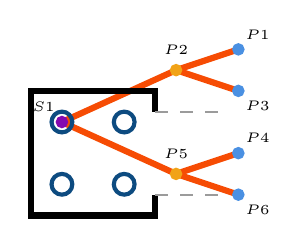
\begin{tikzpicture}[x=0.75pt,y=0.75pt,yscale=-1,xscale=1]
%uncomment if require: \path (0,182); %set diagram left start at 0, and has height of 182

%Straight Lines [id:da47465656152714486] 
\draw [color={rgb, 255:red, 246; green, 76; blue, 4 }  ,draw opacity=1 ][line width=2.25]    (315,75) -- (370,50) ;
%Shape: Square [id:dp7338884259497895] 
\draw  [line width=2.25]  (300,60) -- (360,60) -- (360,120) -- (300,120) -- cycle ;
%Straight Lines [id:da6927342142359094] 
\draw [color={rgb, 255:red, 255; green, 255; blue, 255 }  ,draw opacity=1 ][line width=3]    (360,70) -- (360,110) ;

%Straight Lines [id:da6098087629891208] 
\draw [color={rgb, 255:red, 246; green, 76; blue, 4 }  ,draw opacity=1 ][line width=2.25]    (370,50) -- (400,60) ;
%Straight Lines [id:da9586171017662504] 
\draw [color={rgb, 255:red, 246; green, 76; blue, 4 }  ,draw opacity=1 ][line width=2.25]    (400,40) -- (370,50) ;
%Straight Lines [id:da9166685119570428] 
\draw [color={rgb, 255:red, 246; green, 76; blue, 4 }  ,draw opacity=1 ][line width=2.25]    (370,100) -- (400,110) ;
%Straight Lines [id:da12081008351293132] 
\draw [color={rgb, 255:red, 246; green, 76; blue, 4 }  ,draw opacity=1 ][line width=2.25]    (315,75) -- (370,100) ;
%Straight Lines [id:da43191174777453967] 
\draw [color={rgb, 255:red, 246; green, 76; blue, 4 }  ,draw opacity=1 ][line width=2.25]    (400,90) -- (370,100) ;
%Shape: Circle [id:dp41145059566786146] 
\draw  [color={rgb, 255:red, 132; green, 9; blue, 175 }  ,draw opacity=1 ][fill={rgb, 255:red, 132; green, 9; blue, 175 }  ,fill opacity=1 ] (312.5,75) .. controls (312.5,73.62) and (313.62,72.5) .. (315,72.5) .. controls (316.38,72.5) and (317.5,73.62) .. (317.5,75) .. controls (317.5,76.38) and (316.38,77.5) .. (315,77.5) .. controls (313.62,77.5) and (312.5,76.38) .. (312.5,75) -- cycle ;
%Shape: Circle [id:dp5320458710332802] 
\draw  [color={rgb, 255:red, 13; green, 75; blue, 128 }  ,draw opacity=1 ][line width=1.5]  (310,75) .. controls (310,72.24) and (312.24,70) .. (315,70) .. controls (317.76,70) and (320,72.24) .. (320,75) .. controls (320,77.76) and (317.76,80) .. (315,80) .. controls (312.24,80) and (310,77.76) .. (310,75) -- cycle ;
%Shape: Circle [id:dp3617334287188755] 
\draw  [color={rgb, 255:red, 13; green, 75; blue, 128 }  ,draw opacity=1 ][line width=1.5]  (310,105) .. controls (310,102.24) and (312.24,100) .. (315,100) .. controls (317.76,100) and (320,102.24) .. (320,105) .. controls (320,107.76) and (317.76,110) .. (315,110) .. controls (312.24,110) and (310,107.76) .. (310,105) -- cycle ;
%Shape: Circle [id:dp07731016955749404] 
\draw  [color={rgb, 255:red, 13; green, 75; blue, 128 }  ,draw opacity=1 ][line width=1.5]  (340,105) .. controls (340,102.24) and (342.24,100) .. (345,100) .. controls (347.76,100) and (350,102.24) .. (350,105) .. controls (350,107.76) and (347.76,110) .. (345,110) .. controls (342.24,110) and (340,107.76) .. (340,105) -- cycle ;
%Shape: Circle [id:dp16339127645713447] 
\draw  [color={rgb, 255:red, 13; green, 75; blue, 128 }  ,draw opacity=1 ][line width=1.5]  (340,75) .. controls (340,72.24) and (342.24,70) .. (345,70) .. controls (347.76,70) and (350,72.24) .. (350,75) .. controls (350,77.76) and (347.76,80) .. (345,80) .. controls (342.24,80) and (340,77.76) .. (340,75) -- cycle ;
%Straight Lines [id:da6337075775283348] 
\draw [color={rgb, 255:red, 155; green, 155; blue, 155 }  ,draw opacity=1 ] [dash pattern={on 4.5pt off 4.5pt}]  (360,70) -- (390,70) ;
%Straight Lines [id:da4062260044648891] 
\draw [color={rgb, 255:red, 155; green, 155; blue, 155 }  ,draw opacity=1 ] [dash pattern={on 4.5pt off 4.5pt}]  (360,110) -- (390,110) ;
%Shape: Circle [id:dp34879830519151855] 
\draw  [color={rgb, 255:red, 74; green, 144; blue, 226 }  ,draw opacity=1 ][fill={rgb, 255:red, 74; green, 144; blue, 226 }  ,fill opacity=1 ] (397.5,110) .. controls (397.5,108.62) and (398.62,107.5) .. (400,107.5) .. controls (401.38,107.5) and (402.5,108.62) .. (402.5,110) .. controls (402.5,111.38) and (401.38,112.5) .. (400,112.5) .. controls (398.62,112.5) and (397.5,111.38) .. (397.5,110) -- cycle ;
%Shape: Circle [id:dp05200913272998542] 
\draw  [color={rgb, 255:red, 241; green, 163; blue, 23 }  ,draw opacity=1 ][fill={rgb, 255:red, 241; green, 163; blue, 23 }  ,fill opacity=1 ] (367.5,100) .. controls (367.5,98.62) and (368.62,97.5) .. (370,97.5) .. controls (371.38,97.5) and (372.5,98.62) .. (372.5,100) .. controls (372.5,101.38) and (371.38,102.5) .. (370,102.5) .. controls (368.62,102.5) and (367.5,101.38) .. (367.5,100) -- cycle ;
%Shape: Circle [id:dp43357034961897] 
\draw  [color={rgb, 255:red, 74; green, 144; blue, 226 }  ,draw opacity=1 ][fill={rgb, 255:red, 74; green, 144; blue, 226 }  ,fill opacity=1 ] (397.5,40) .. controls (397.5,38.62) and (398.62,37.5) .. (400,37.5) .. controls (401.38,37.5) and (402.5,38.62) .. (402.5,40) .. controls (402.5,41.38) and (401.38,42.5) .. (400,42.5) .. controls (398.62,42.5) and (397.5,41.38) .. (397.5,40) -- cycle ;
%Shape: Circle [id:dp7842924247669173] 
\draw  [color={rgb, 255:red, 241; green, 163; blue, 23 }  ,draw opacity=1 ][fill={rgb, 255:red, 241; green, 163; blue, 23 }  ,fill opacity=1 ] (367.5,50) .. controls (367.5,48.62) and (368.62,47.5) .. (370,47.5) .. controls (371.38,47.5) and (372.5,48.62) .. (372.5,50) .. controls (372.5,51.38) and (371.38,52.5) .. (370,52.5) .. controls (368.62,52.5) and (367.5,51.38) .. (367.5,50) -- cycle ;
%Shape: Circle [id:dp5315495156196338] 
\draw  [color={rgb, 255:red, 74; green, 144; blue, 226 }  ,draw opacity=1 ][fill={rgb, 255:red, 74; green, 144; blue, 226 }  ,fill opacity=1 ] (397.5,60) .. controls (397.5,58.62) and (398.62,57.5) .. (400,57.5) .. controls (401.38,57.5) and (402.5,58.62) .. (402.5,60) .. controls (402.5,61.38) and (401.38,62.5) .. (400,62.5) .. controls (398.62,62.5) and (397.5,61.38) .. (397.5,60) -- cycle ;
%Shape: Circle [id:dp9788740260400791] 
\draw  [color={rgb, 255:red, 74; green, 144; blue, 226 }  ,draw opacity=1 ][fill={rgb, 255:red, 74; green, 144; blue, 226 }  ,fill opacity=1 ] (397.5,90) .. controls (397.5,88.62) and (398.62,87.5) .. (400,87.5) .. controls (401.38,87.5) and (402.5,88.62) .. (402.5,90) .. controls (402.5,91.38) and (401.38,92.5) .. (400,92.5) .. controls (398.62,92.5) and (397.5,91.38) .. (397.5,90) -- cycle ;

% Text Node
\draw (313,71.6) node [anchor=south east] [inner sep=0.75pt]  [font=\tiny]  {$S1$};
% Text Node
\draw (370,44.1) node [anchor=south] [inner sep=0.75pt]  [font=\tiny]  {$P2$};
% Text Node
\draw (402,36.6) node [anchor=south west] [inner sep=0.75pt]  [font=\tiny]  {$P1$};
% Text Node
\draw (402,63.4) node [anchor=north west][inner sep=0.75pt]  [font=\tiny]  {$P3$};
% Text Node
\draw (402,86.6) node [anchor=south west] [inner sep=0.75pt]  [font=\tiny]  {$P4$};
% Text Node
\draw (370,94.1) node [anchor=south] [inner sep=0.75pt]  [font=\tiny]  {$P5$};
% Text Node
\draw (402,113.4) node [anchor=north west][inner sep=0.75pt]  [font=\tiny]  {$P6$};


\end{tikzpicture}
    \vspace{-1cm}
    \caption{Outcome state after implementing \cref{eq:tree_implementation}}
    \label{fig:final_tree_implementation}
\end{figure}